% Compile with Tectonic:
%   conda run -n alphagenome tectonic docs/rna_seq11_collaborator_update_20260604.tex
\documentclass[UTF8,aspectratio=169,10pt]{ctexbeamer}

\usetheme{Boadilla}
\usecolortheme{dolphin}
\setbeamertemplate{navigation symbols}{}
\setbeamertemplate{footline}[frame number]

\usepackage{booktabs}
\usepackage{array}
\usepackage{tikz}
\usepackage{pgfplots}
\usetikzlibrary{arrows.meta,positioning}
\pgfplotsset{compat=1.18}

\definecolor{agblue}{RGB}{38,88,156}
\definecolor{aggreen}{RGB}{37,125,97}
\definecolor{agred}{RGB}{174,74,65}
\definecolor{aggray}{RGB}{92,102,112}
\definecolor{agpurple}{RGB}{106,83,155}

\setbeamercolor{title}{fg=agblue}
\setbeamercolor{frametitle}{fg=agblue}
\setbeamercolor{structure}{fg=agblue}
\setbeamercolor{block title}{fg=white,bg=agblue!82}
\setbeamercolor{block body}{bg=agblue!5}

\title[C. elegans RNA-seq Adapter Update]{C. elegans 11-track RNA-seq\\AlphaGenome Adapter Update}
\subtitle{实验版本、结果、diagnostics 与下一步判断}
\author{Ziyang Huang}
\date{2026-06-04}

\newcommand{\smallnote}[1]{\vspace{0.35em}{\scriptsize\color{aggray}#1}}
\newcommand{\code}[1]{\texttt{\scriptsize #1}}

\begin{document}

\begin{frame}
  \titlepage
\end{frame}

\begin{frame}{这份 slides 怎么读}
  \begin{block}{我把长 checkpoint 名改成了短代号}
    \begin{tabular}{lll}
      \toprule
      Prefix & Meaning & Examples \\
      \midrule
      A & 128 bp adapter 系列 & A0, A1, A2 \\
      B & 1 bp-B residual correction 系列 & B0, B1 \\
      S & signal-weighted loss 系列 & S1, S2, S3 \\
      R & region-weighted loss 系列 & R1, R2 \\
      G & gene auxiliary loss 系列 & G1, G2 \\
      K & calibration 系列 & K1, K2 \\
      P & downstream probe / representation 参考 & P1 \\
      \bottomrule
    \end{tabular}
  \end{block}

  \begin{itemize}
    \item 正文只用短代号，方便听汇报。
    \item 最后 appendix 给出短代号到完整 run directory 的对应关系。
    \item 所有新结果都是 validation-only；没有继续用 test 选模型。
  \end{itemize}
\end{frame}

\begin{frame}{从上次 PPT 到现在：我实际多跑了什么}
  \begin{center}
  \begin{tabular}{p{0.16\textwidth}p{0.34\textwidth}p{0.38\textwidth}}
    \toprule
    Stage & Ran & What it answered \\
    \midrule
    A-series & 128 bp head/loss/schedule sweep & 128 bp baseline 还能不能明显提高？ \\
    B-series & 1 bp residual correction & 1 bp embeddings 是否能在 128 bp base 上补信号？ \\
    Diagnostics & top15 extended diagnostics & 当前 best 模型到底弱在哪里？ \\
    S/R/G/K & signal, region, gene-aux, calibration & 能否针对 high-signal / exon / gene-level / amplitude 修正？ \\
    All-model eval & 171 个已训模型全量重测 & 如果不只看 MSE，哪个模型更有生物 utility？ \\
    Probe & gene-profile downstream probe & 输出里是否保留 gene-level / track-level 可用结构？ \\
    \bottomrule
  \end{tabular}
  \end{center}
\end{frame}

\begin{frame}{数据和约束没有变}
  \begin{columns}[T,onlytextwidth]
    \begin{column}{0.47\textwidth}
      \begin{itemize}
        \item Reference: C. elegans WBcel235
        \item 20 sample-level RNA-seq bigWig
        \item grouped into 11 RNA-seq tracks
        \item window: 1,048,576 bp
        \item stride: 524,288 bp
        \item target: log1p RNA-seq signal
      \end{itemize}
    \end{column}
    \begin{column}{0.48\textwidth}
      \centering
      \begin{tabular}{lcc}
        \toprule
        Split & Chromosome & NPZ \\
        \midrule
        Train & I--IV & 116 \\
        Valid & V & 39 \\
        Test & X & 33 \\
        \bottomrule
      \end{tabular}

      \vspace{0.8em}
      \begin{block}{Rule}
        后续所有训练、筛选、diagnostics 都只用 train/valid。\\
        Test 没有继续用于调参。
      \end{block}
    \end{column}
  \end{columns}
\end{frame}

\begin{frame}{A-series: 128 bp 后续 sweep}
  \centering
  \begin{tabular}{llccc}
    \toprule
    ID & Version & Valid MSE & MAE & Pearson \\
    \midrule
    A0 & 5/18 128 bp baseline & 1.0609935 & 0.718662 & 0.588099 \\
    A1 & residual-conv3 sweep winner & 0.9079802 & 0.589446 & 0.663840 \\
    A2 & Phase4 conv5 step4000 winner & \textbf{0.8803258} & \textbf{0.584829} & \textbf{0.673917} \\
    \bottomrule
  \end{tabular}

  \vspace{1em}
  \begin{block}{Analysis}
    128 bp 不是已经到头。更合适的 head、full-log1p target、hybrid/SmoothL1 loss 和 LR schedule 把 valid MSE 从 1.06 推到 0.88。
  \end{block}

  \smallnote{A2 后来作为 1 bp residual correction 的 frozen base。}
\end{frame}

\begin{frame}{A-series: MSE 变化图}
  \centering
  \begin{tikzpicture}
    \begin{axis}[
      width=0.88\textwidth,
      height=0.58\textheight,
      ybar,
      ymin=0.82,
      ymax=1.10,
      ylabel={Valid full MSE},
      symbolic x coords={A0,A1,A2},
      xtick=data,
      bar width=26pt,
      nodes near coords,
      nodes near coords style={font=\scriptsize,anchor=south},
      every axis plot/.append style={fill=agblue!30,draw=agblue!60}
    ]
      \addplot coordinates {(A0,1.0609935) (A1,0.9079802) (A2,0.8803258)};
    \end{axis}
  \end{tikzpicture}

  \smallnote{这一步回答：旧 PPT 的 128 bp baseline 不是最终水平。}
\end{frame}

\begin{frame}{B-series: 1 bp-B residual correction}
  \centering
  \begin{tabular}{llcccc}
    \toprule
    ID & Version & Full MSE & MAE & Pearson & common128 MSE \\
    \midrule
    A2 & 128 bp frozen base & 0.8803258 & 0.584829 & 0.673917 & 0.868292 \\
    B0 & 1 bp-B rank1 & \textbf{0.8355771} & \textbf{0.581805} & \textbf{0.694634} & 0.837371 \\
    B1 & 1 bp-B rank3 & 0.8356444 & 0.582023 & 0.694629 & \textbf{0.837121} \\
    \bottomrule
  \end{tabular}

  \vspace{1em}
  \begin{block}{Analysis}
    1 bp embedding 的 residual correction 是有用的：相对 A2，B0 valid MSE 降了约 0.04475，Pearson 增加约 0.02072。
  \end{block}

  \smallnote{B0 是当前 full-MSE reference；B1 是 gene/pooled metrics 的 co-reference。}
\end{frame}

\begin{frame}{B-series top15: 进入 plateau}
  \begin{columns}[T,onlytextwidth]
    \begin{column}{0.48\textwidth}
      \begin{block}{top15 共同模式}
        \begin{itemize}
          \item 都是 A2 frozen 128 bp prediction
          \item 加 1 bp residual correction
          \item 主要差别：warm-start、LR、beta、track weights
          \item top15 full-MSE spread 约 0.00137
        \end{itemize}
      \end{block}
    \end{column}
    \begin{column}{0.48\textwidth}
      \begin{block}{剩余弱点}
        \begin{itemize}
          \item high-signal / top1 / top5 amplitude
          \item exon / gene-body
          \item intestine T1/T3/T4
          \item gene-level expression
          \item 1 bp local-gradient / boundary
        \end{itemize}
      \end{block}
    \end{column}
  \end{columns}

  \vspace{0.6em}
  \smallnote{这一步回答：继续同方向小调参收益很小，要开始按弱点设计实验。}
\end{frame}

\begin{frame}{Diagnostics: B0 的具体弱点}
  \centering
  \begin{tabular}{lcc}
    \toprule
    Metric & B0 value & Meaning \\
    \midrule
    high\_gt3 MSE & 4.9257 & high expression amplitude weak \\
    top5 true MSE & 5.8610 & top 5\% true signal weak \\
    top1 true MSE & 10.8414 & extreme peaks weak \\
    exon MSE & 1.6658 & exon region error high \\
    gene-body MSE & 1.1104 & gene-body signal not solved \\
    gene Spearman & 0.5835 & gene rank partially preserved \\
    local-gradient Pearson & 0.3451 & local boundary shape weak \\
    \bottomrule
  \end{tabular}

  \vspace{0.8em}
  \begin{block}{Analysis}
    B0 的全局 MSE 很好，但 biologically important high-expression / gene-body / intestine signal 还没有完全学好。
  \end{block}
\end{frame}

\begin{frame}{S-series: signal-weighted loss}
  \centering
  \begin{tabular}{llcccc}
    \toprule
    ID & Version & Full MSE & high\_gt3 & top5 & top1 \\
    \midrule
    B0 & reference & \textbf{0.8356} & 4.9257 & 5.8610 & 10.8414 \\
    S1 & top1x5, low LR & 0.8450 & 4.4820 & 5.2960 & 9.8991 \\
    S2 & top5x3 & 0.8632 & \textbf{4.1605} & \textbf{4.9061} & \textbf{9.2685} \\
    S3 & intestine-highx3 & 0.8531 & 4.3510 & 5.1905 & 9.8277 \\
    \bottomrule
  \end{tabular}

  \vspace{0.8em}
  \begin{block}{Analysis}
    Signal weighting 确实能修 high-signal amplitude；代价是 full MSE 变差。它们不适合作为唯一主模型，但适合保留为 high-expression / intestine co-winner。
  \end{block}
\end{frame}

\begin{frame}{R-series: region-weighted loss}
  \centering
  \begin{tabular}{llccccc}
    \toprule
    ID & Version & Full MSE & Exon & Gene-body & Intergenic & Rep score \\
    \midrule
    B0 & reference & \textbf{0.8356} & 1.6658 & 1.1104 & \textbf{0.2980} & 0.8176 \\
    R1 & exon-gene v2 & 0.8367 & 1.6591 & 1.1083 & 0.3048 & \textbf{0.8881} \\
    R2 & exon-gene v1 & 0.8377 & \textbf{1.6550} & \textbf{1.1079} & 0.3084 & 0.8317 \\
    \bottomrule
  \end{tabular}

  \vspace{0.8em}
  \begin{block}{Analysis}
    Region weighting 的效果是清楚的：exon/gene-body 下降，但 intergenic 变差。R2 是最强 region winner；R1 是最平衡的 representation winner。
  \end{block}
\end{frame}

\begin{frame}{G/K-series: gene auxiliary 与 calibration}
  \centering
  \begin{tabular}{llcccc}
    \toprule
    ID & Version & Full MSE & Gene MSE & Gene Spearman & high\_gt3 \\
    \midrule
    B0 & reference & \textbf{0.835577} & \textbf{0.712698} & 0.583460 & 4.9257 \\
    G1 & gene-aux $\lambda=0.03$ & 0.835827 & 0.713353 & 0.583523 & 4.9179 \\
    G2 & R1 + gene-aux $\lambda=0.03$ & 0.837019 & 0.715049 & 0.584113 & 4.8248 \\
    K1 & track-affine lr3e-5 & 0.835773 & 0.712705 & 0.583438 & 4.9120 \\
    K2 & track-affine lr1e-4 & 0.836070 & 0.712741 & 0.583378 & 4.8931 \\
    \bottomrule
  \end{tabular}

  \vspace{0.8em}
  \begin{block}{Analysis}
    Gene-aux 和 calibration 都有小信号，但没有形成新的主 winner。Calibration 轻微改善 amplitude；gene-aux 没有改善 gene MSE。
  \end{block}
\end{frame}

\begin{frame}{Intestine T1/T3/T4 专项}
  \centering
  \begin{tabular}{llccc}
    \toprule
    ID & Version & T1/T3/T4 high\_gt3 & T1/T3/T4 gene Spearman & Full MSE \\
    \midrule
    B0 & reference & 5.2666 & 0.5460 & \textbf{0.8356} \\
    R1 & region v2 & 5.1702 & 0.5469 & 0.8367 \\
    S2 & top5x3 & 4.4794 & \textbf{0.5513} & 0.8632 \\
    S3 & intestine-highx3 & \textbf{4.4591} & 0.5513 & 0.8531 \\
    \bottomrule
  \end{tabular}

  \vspace{0.8em}
  \begin{block}{Analysis}
    Intestine 的 high-expression signal 更偏向 S-series。也就是说 full MSE 会惩罚它们，但它们确实学到了 B0 没表达好的 intestine 强信号。
  \end{block}
\end{frame}

\begin{frame}{Gene-level / pooled / boundary diagnostics}
  \centering
  \begin{tabular}{llccccc}
    \toprule
    ID & Version & Gene MSE & Gene Sp. & 128bp MSE & 1kb MSE & Gradient P. \\
    \midrule
    B0 & rank1 & 0.7127 & 0.5835 & 0.7202 & 0.5451 & \textbf{0.3451} \\
    B1 & rank3 & \textbf{0.7126} & 0.5837 & \textbf{0.7201} & \textbf{0.5451} & 0.3446 \\
    R1 & region v2 & 0.7148 & \textbf{0.5840} & 0.7213 & 0.5466 & 0.3431 \\
    \bottomrule
  \end{tabular}

  \vspace{0.8em}
  \begin{block}{Analysis}
    B1 是 gene/pooled co-reference。Local-gradient 没有被任何新 objective 明显修好，说明边界/高频形状可能需要结构层面的改变。
  \end{block}
\end{frame}

\begin{frame}{All-model evaluation: 171 个已训模型重新测评}
  \begin{block}{这一步不是重新训练主模型}
    \begin{itemize}
      \item 从 runs/ 中收集 171 个已有 checkpoint。
      \item 对每个模型在 valid chr V 上重新跑 extended diagnostics。
      \item 对每个模型提取 train/valid gene-level predicted profiles。
      \item 训练 lightweight downstream probe：只用 train chromosomes，在 chr V 验证。
    \end{itemize}
  \end{block}

  \begin{block}{Why}
    我们想回答：哪个模型更会找 biologically important signal，而不是哪个模型 pixel-level MSE 最低。
  \end{block}
\end{frame}

\begin{frame}{All-model evaluation: 结果}
  \centering
  \begin{tabular}{llll}
    \toprule
    Role & ID & Version & Key number \\
    \midrule
    MSE reference & B0 & 1 bp-B rank1 & full MSE 0.8356 \\
    Representation winner & R1 & region v2 & rep score 0.8881 \\
    Region winner & R2 & region v1 & exon/gene-body best \\
    High-signal winner & S2 & top5x3 & top1 MSE 9.2685 \\
    Intestine winner & S3 & intestine-highx3 & T1/T3/T4 high\_gt3 4.4591 \\
    Probe co-reference & P1 & broad w5 & probe score 0.8581 \\
    \bottomrule
  \end{tabular}

  \vspace{0.8em}
  \begin{block}{Analysis}
    现在最合理的汇报方式不是单一 winner，而是 winner set：B0 做 MSE reference；R1 做主 representation candidate；S2/S3 做 high-expression/intestine co-winner。
  \end{block}
\end{frame}

\begin{frame}{Downstream probe: 结果怎么解释}
  \centering
  \begin{tabular}{llccc}
    \toprule
    ID & Version & top5 gene recall & T1/T3/T4 recall & track corr Sp. \\
    \midrule
    B0 & rank1 & 0.4991 & 0.4684 & 0.8771 \\
    R1 & region v2 & 0.4999 & 0.4694 & \textbf{0.8778} \\
    S2 & top5x3 & \textbf{0.5017} & 0.4713 & 0.8760 \\
    P1 & broad w5 & 0.4985 & 0.4694 & 0.8768 \\
    \bottomrule
  \end{tabular}

  \vspace{0.8em}
  \begin{block}{Analysis}
    Probe 差距不大，所以不能单独决定模型。但它支持一个判断：S-series 对 top expressed gene retrieval 有帮助；R1 是更平衡的 overall choice。
  \end{block}
\end{frame}

\begin{frame}{最终我会怎么给合作者解释}
  \begin{itemize}
    \item 5/18 的 A0 baseline 已经过时：128 bp 后续优化到 A2，1 bp residual 到 B0。
    \item B0 是当前 pixel-level full-MSE reference。
    \item Diagnostics 显示 B0 的弱点集中在 high-signal amplitude、exon/gene-body、intestine T1/T3/T4 和 local boundary。
    \item S-series 证明 high-expression amplitude 可以被修，但 full MSE 会变差。
    \item R-series 证明 exon/gene-body 可以被修；R1 是最平衡的 representation candidate。
    \item 171-model benchmark 和 probe 让我们从“刷 MSE”转成“按生物 utility 选模型”。
  \end{itemize}
\end{frame}

\begin{frame}{Next steps}
  \begin{columns}[T,onlytextwidth]
    \begin{column}{0.48\textwidth}
      \begin{block}{Model side}
        \begin{itemize}
          \item 保留 B0 作为 MSE reference
          \item 用 R1 做 main representation candidate
          \item 用 S2/S3 做 high-expression/intestine co-winner
          \item 下一步尝试 amplitude calibration / target parameterization
        \end{itemize}
      \end{block}
    \end{column}
    \begin{column}{0.48\textwidth}
      \begin{block}{Evaluation side}
        \begin{itemize}
          \item 固定 gene retrieval 作为 downstream metric
          \item 单独跟踪 intestine T1/T3/T4
          \item local-gradient 作为 boundary diagnostic
          \item 暂时不碰 test split
        \end{itemize}
      \end{block}
    \end{column}
  \end{columns}
\end{frame}

\begin{frame}{Appendix: version mapping 1}
  \footnotesize
  \begin{tabular}{p{0.08\textwidth}p{0.25\textwidth}p{0.56\textwidth}}
    \toprule
    ID & Short name & Human-readable version \\
    \midrule
    A0 & 5/18 128 bp baseline & formal 128 bp adapter, 5000 steps, lr $3e{-4}$ \\
    A1 & residual-conv3 sweep & 128 bp residual-conv3, full-log1p, SmoothL1, lr $1e{-3}$ \\
    A2 & 128 bp Phase4 conv5 & 128 bp conv5 h256, hybrid loss, step LR decay at step 4000 \\
    B0 & 1 bp-B rank1 & frozen A2 base + 1 bp residual conv5, hard15, beta0.5, lr $1e{-5}$ \\
    B1 & 1 bp-B rank3 & same family as B0, different warm-start / track-weight setting \\
    \bottomrule
  \end{tabular}

  \smallnote{Exact run directories are recorded in docs/rna\_seq11\_adaptive\_objective\_screen\_20260529.md and docs/rna\_seq11\_all\_representation\_utility\_20260530.md.}
\end{frame}

\begin{frame}{Appendix: version mapping 2}
  \footnotesize
  \begin{tabular}{p{0.08\textwidth}p{0.25\textwidth}p{0.56\textwidth}}
    \toprule
    ID & Short name & Human-readable version \\
    \midrule
    S1 & signal top1x5 & B0 warm-start, hybrid alpha0.75 beta0.5, top1 signal weighted $5\times$, lr $3e{-6}$ \\
    S2 & signal top5x3 & B0 warm-start, top5 signal weighted $3\times$, lr $1e{-5}$ \\
    S3 & signal intestine-high & B0 warm-start, intestine high-signal weighted $3\times$, lr $1e{-5}$ \\
    R1 & region exon-gene v2 & B0 warm-start, exon/gene-body/promoter weighted gently, 1000 steps \\
    R2 & region exon-gene v1 & B0 warm-start, stronger exon/gene-body weighting, 1500 steps \\
    \bottomrule
  \end{tabular}
\end{frame}

\begin{frame}{Appendix: version mapping 3}
  \footnotesize
  \begin{tabular}{p{0.08\textwidth}p{0.25\textwidth}p{0.56\textwidth}}
    \toprule
    ID & Short name & Human-readable version \\
    \midrule
    G1 & gene-aux rank1 & B0 warm-start + gene-body mean auxiliary loss $\lambda=0.03$ \\
    G2 & region v2 + gene-aux & R1 warm-start + gene-body mean auxiliary loss $\lambda=0.03$ \\
    K1 & track-affine lr3e-5 & B0 + identity-initialized per-track affine output calibration \\
    K2 & track-affine lr1e-4 & same as K1 but higher LR and shorter run \\
    P1 & probe co-reference & 1 bp-B broad w5 checkpoint; strongest near-frontier downstream-probe score \\
    \bottomrule
  \end{tabular}
\end{frame}

\end{document}
